\documentclass[twocolumn]{article}
\usepackage{PRIMEarxiv}

\usepackage[utf8]{inputenc} % allow utf-8 input
\usepackage[T1]{fontenc}    % use 8-bit T1 fonts
\usepackage{hyperref}       % hyperlinks
\usepackage{url}            % simple URL typesetting
\usepackage{booktabs}       % professional-quality tables
\usepackage{amsfonts}       % blackboard math symbols
\usepackage{amsmath}
\usepackage{amsthm}


\usepackage{natbib}

\usepackage{multirow}

\usepackage{algorithm}
\usepackage{algpseudocode}

\usepackage{tikz}
\usetikzlibrary{quantikz2}

\usepackage{nicefrac}       % compact symbols for 1/2, etc.
\usepackage{microtype}      % microtypography
\usepackage{cuted}
\usepackage{fancyhdr}       % header
\usepackage{graphicx}       % graphics
\usepackage{subfig}

\graphicspath{{images/}}     % organize your images and other figures under media/ folder

\usepackage{multicol}
\usepackage{tcolorbox}
%Header
\pagestyle{fancy}
\thispagestyle{empty}
\rhead{ \textit{ }} 

% Update your Headers here
\fancyhead[LO]{Convolution}
% \fancyhead[RE]{Firstauthor and Secondauthor} % Firstauthor et al. if more than 2 - must use \documentclass[twoside]{article}


\newtheorem*{note}{Note}
  

\newtheorem{theorem}{Theorem}
\tcolorboxenvironment{theorem}{
    colback=blue!5!white,
    boxrule = 0.2pt,
    boxsep=1pt,
    left= 2pt, right=2pt, top=2pt, bottom=2pt,
    oversize = 1.5pt,
    sharp corners, 
    before skip = \topsep,
    after skip = \topsep
}



%% Title
\title{Spectrum search algorithm on Quantum computation
%%%% Cite as
%%%% Update your official citation here when published 
%\thanks{\textit{\underline{Citation}}: 
%\textbf{Authors. Title. Pages.... DOI:000000/11111.}} 
}

\author{
    \href{https://orcid.org/0000-0002-4876-7820}{
        
\includegraphics[scale=0.06]{orcid.pdf}\hspace{1mm}Hyunseong Kim}\\
  Department of Physics and Photon Science,  \\
  Gwangju Institute of Science and Technology\\
  Gwangju\\
  \texttt{qwqwhsnote@gm.gist.ac.kr} \\
  %% examples of more authors
  %% \AND
  %% Coauthor \\
  %% Affiliation \\
  %% Address \\
  %% \texttt{email} \\
  %% \And
  %% Coauthor \\
  %% Affiliation \\
  %% Address \\
  %% \texttt{email} \\
  %% \And
  %% Coauthor \\
  %% Affiliation \\
  %% Address \\
  %% \texttt{email} \\
}

\begin{document}
\twocolumn[ 
\begin{@twocolumnfalse}
    \begin{center}

    \maketitle

\begin{abstract}
Spectrum search algorithm was designed by combining imaginary time evolution and Grover search algorithm.
The Grover algorithm was used to eliminate the known states from the fully-mixed state.
By iteratively applying the eilination algorithm and imaginary evolution, we can obtain 
full spectrum of the general Hamiltonian including degeneracy states.
\end{abstract}

% keywords can be removed
\keywords{Spectrum search \and Imaginary time evloution \and Grover algorithm \and Quantum simulation}
    \end{center}
\end{@twocolumnfalse}
]

%\begin{multicols*}{2}
    

\section{Introduction}
Spectrum search is a fundamental routine in physics to analysis 
the given quantum system. 
In the research, two algorithms were combined 
to construct the spectrum search algorithm of the given quantum system;
imaginary time evolution, and Grover search algorithm.
Theoretically, the composed algorithm aims the time-independent
Hamiltonian system, and could measure the full spectrum of the system
by iteratively applying the algorithm from the ground to the higher energy state
, without affected by degeneracy of the system.

\begin{figure}[!ht]
    \centering
    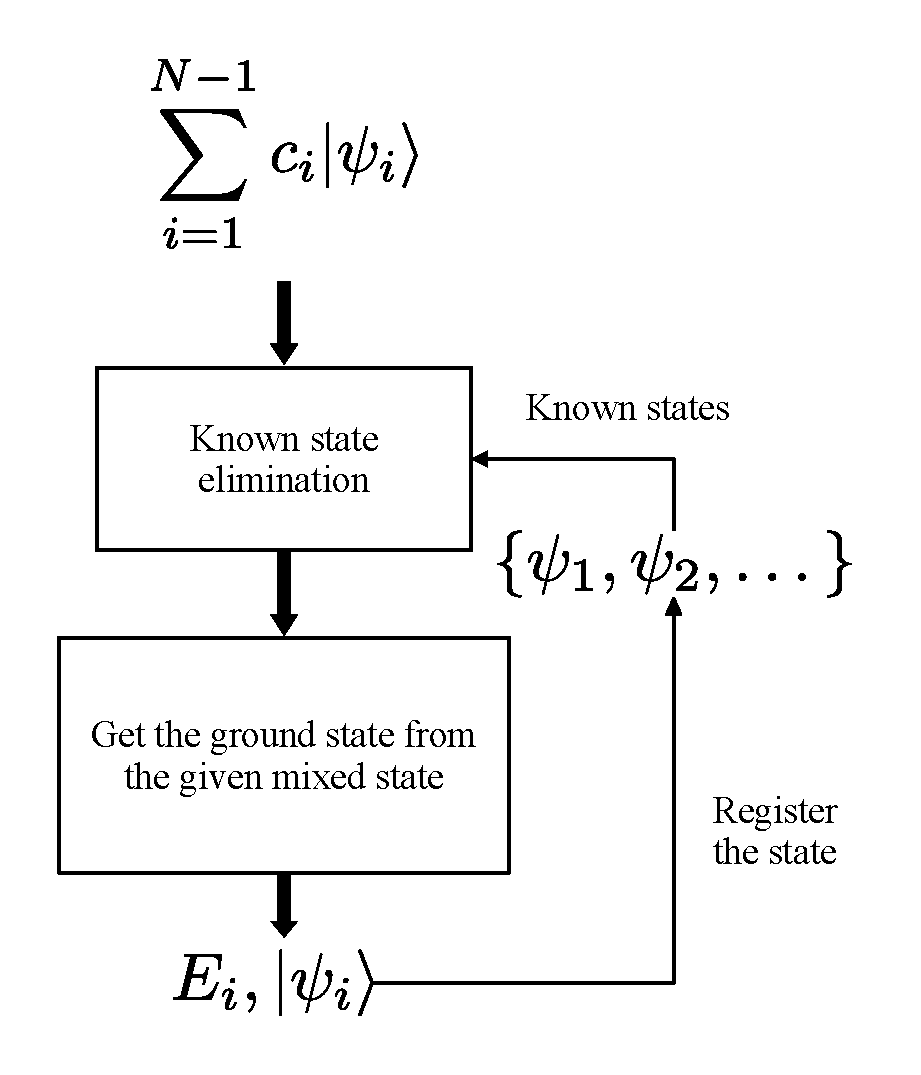
\includegraphics[width=\linewidth]{Algorithm_diagram.pdf}
    \caption{Schematics of the algorithm flow.}
    \label{fig:alg_flow}
\end{figure}
%-------------------------------------------

\section{Background knowledges}

\subsection{Spectrum theory}

In the finite dimension, any given system Hamiltonians has a finite Hermit matrix form,
and their time evolution operator is unitary, $U$, with 

\begin{equation}
    U = e^{-i H t}
\end{equation}
form.

\begin{theorem}
    For a given Hermit matrix $H$ and eigen vector, $\mathbf{v}$ with
    \begin{equation}
        H \mathbf{v} = \lambda \mathbf{v}
    \end{equation}
    then, $\mathbf{v}$ is an eigenvector of the unitary matrix, $U = \exp(-i H)$ and 
    its eigen values is $\exp(-i \lambda)$.

    \begin{equation}
        \exp(-i H) \mathbf{v} = \exp(-i \lambda) \mathbf{v}
    \end{equation}
\end{theorem}

\begin{theorem}{Spectrum theorem}
    
    \begin{itemize}
        \item For a given Hermit matrix $H$, it has an orthonormal eigen-basis.
        \item For a given Unitary matrix $U$, it has an orthonormal eigen-basis.
    \end{itemize}

\end{theorem}

The orthogonality plays significant role in the below section.
All state we want to find is mutually orthogonal to each other.

\subsection{Imaginary quantum evolution}

Imaginary time evolution is frequently used in 
quantum system simulation in statistical physics. 
The reason is that from the given governing equation; Schr$\ddot{\mbox{o}}$dinger  equation,
we can directly obtain a progress to reach the ground state of the system.
From the time-independent Schr$\ddot{\mbox{o}}$dinger  equation, 

\begin{equation}
    i \hbar \frac{\partial}{\partial}| \psi \rangle = H |\psi \rangle
\end{equation}

takes $\tau = i t$  then, $df/d\tau = (dt/d\tau) df/dt = i df/dt$, thus,

\begin{align}
    \frac{\partial}{\partial \tau} | \psi \rangle = H | \psi \rangle \label{eq:imginary_sch_eq}\\
    | \psi(\tau) \rangle = e^{- \tau H} | \psi(0) \rangle
\end{align}

From the Eq (\ref{eq:imginary_sch_eq}), we get a general solution,

\begin{equation}
    |\Psi \rangle = \sum_{i} c_i(0) e^{- E_i \tau} | \psi_i \rangle
\end{equation}

The terms are decaying and does not oscillate. Therefore, with sufficient long time, $\tau$, 
we get 

\begin{equation}
    |\Psi(\tau) \approx_{\tau \rightarrow \infty} c_g(0) e^{- E_g \tau} | \psi_g \rangle
\end{equation}

However, the imaginary time evolution cannot be directly 
implemented in common gate model computer. 
Since, it is a non-unitary transformation, $\exp(-H \tau)^\dagger = \exp(-H \tau)$, Hermit. 
Therefore, the implementation of ITE is also a challenge in the quantum computation.
There are several ways, one is approximate the non-unitary gate with unitary gate.
It is a common method by VQE, we can approximate unitary process to reach the same result 
of the imaginary time steps. 
The other methods are a block-encoding, embeding the non-unitary gate into unitary gate, or
using a measurement based approach. 
The method we used in the implementation was non-unitary Trotter circuit suggested by Leadbeater et al\cite{leadbeater_non-unitary_2023}.
Once we get a proper ITE routine, then the quantum computer could find a ground state from 
the \textit{given} states.

\subsection{Mixed state}

There weakness also arise from that if the ground state was not in the 
given mixed state, one cannot find the proper ground state.
Even the state is mixed completely in computational basis,
in the eigen basis of the Hamiltonian, it could be just a few combination
or a basis itself.
For example, $\frac{1}{\sqrt{2}}(|0\rangle + |1\rangle)^{\otimes n}$
has full eigen states of the $n$-qubit system in computational basis, 
however, for $H= \sum_i X^i$. It is just an eigen-basis with ground energy.

The fully mixed state representation in computational basis 
is not hard to obtain, just add all column of the given matrix, 
we get a fully mixed state in the eigen basis of the matrix.
Unfortunately, the preparation of the such state on QC is an another 
challenge, and this topic would not be analyzed in this research.


Even though the mixed state preparation problem, the property of the ITE is very powerful. 
Without changing the Hamiltonian,
if the given state only consists of excited states of the system, 
we get a lowest energy state and it would be a specific excited state of 
the original Hamiltonian.
For example, If we want to get a 2nd excited state from the system, 
only thing we have to do is preparing the mixed state in which the ground and 1st excited states are not combined
and just apply the ITE routine.
Thus, if we can efficiently eliminate the known ground states from 
the mixed state, we have a spectrum search algorithm with imaginary time evolution.
We already know the algorithm modifying amplitude of state to the desired state, \textit{Grover algorithm}.

%\subsection{Grover Search algorithm}

\section{Spectrum Search algorithm}

In the original Grover algorithm, 
the object was search the proper state,
however, in here our object is
\textit{eliminating the known state} from 
the given mixed state.
More specificially, if the eigen-states of the given Hamiltonain, $H$,
was $\{|\psi_i \rangle \}_{i=1}^n$,
and we know $|\psi_1 \rangle$,
we want to get the next state 

\begin{equation}
    |\Psi\rangle = \sum_{i \neq 1} c_i | \psi_i \rangle \, , c_i \neq \forall i
\end{equation}

$|\Psi\rangle$ and $|\psi_1\rangle$ are orthonormal by the spectrum theorem of Hermit matrix.
If we have a proper oracle gate, we can obtain the $|\Psi\rangle$ state by using Grover iteration.
In fact, the oracle gate in the situation is defined with $e(iH')$ form, naturally.

\subsection{Qauntnum oracle}

With the given ground state, $| \psi_g\rangle$, and the combination of all the other 
specturm, $|\Psi \rangle$, define a $H'$ as 

\begin{equation}
    \label{eq:grover_H_def}
    H' = I - | \psi_g \rangle \langle \psi_g|
\end{equation}

then, 

\begin{equation}
    H' |\psi \rangle = \begin{cases}
        0 |\psi \rangle & \text{if }  |\psi \rangle = |\psi_g \rangle\\
        1 |\psi \rangle & \text{if }  |\psi \rangle = |\Psi \rangle
    \end{cases}
\end{equation}

and by the Theorem 1,

\begin{equation}
    \label{eq:oracle_def_eq}
    \exp(i \pi H') |\psi \rangle = \begin{cases}
        1 |\psi \rangle & \text{if }  |\psi \rangle = |\psi_g \rangle\\
        -1 |\psi \rangle & \text{if }  |\psi \rangle = |\Psi \rangle
    \end{cases}
\end{equation}

The state $|\Psi \rangle$ is a state we want to get 
after the Grover iteration. Therefore, Eq (\ref{eq:oracle_def_eq}) satisfies 
the oracle gate required in the iteration. In addition, the implementation of the oracle is 
well-analyed already; Trotterization.

\begin{equation}
    U_\omega = \exp(- i \pi (I-| \psi_g \rangle \langle \psi_g|) )
\end{equation}

However, the Grover algorithm only increases the probability to be orthogonal
to the given state. For the precise spectrum search, we have to ensure the perfectly 
orthogonal to the known state, unless we still get a same ground state by ITE.

\subsection{Measurement}

Consider the POM, $M_0 = |\psi_0 \rangle \langle \psi_0|$, 
after the measurement, the remained state would be 

\begin{equation}
    \frac{M_0 |\psi \rangle}{\sqrt{\langle \psi |M_0^\dagger M_0|\psi \rangle}} = \begin{cases}
        |\psi_g \rangle & \text{if } \langle M_0 \rangle \neq 0\\
        |\Psi \rangle & \text{if } \langle M_0 \rangle = 0
    \end{cases}
\end{equation}

thus, applying the $M_0$ to get a 0 value, we can ensure the $|\psi_0\rangle$ 
is totally eliminated from the state.
The remaning thing is applying the imaginary evolution, we will get a 
1st exicted state or, if the system has a degeneracy in the ground state,
we get an another ground state.

\subsection{i-th state}

By iteratively applying the result, we want the algorithm to 
eliminate the state from the mixed state and get full-eigen state.

\begin{equation}
    \begin{array}{l}
        [ \{\psi_1, \psi_2 , \psi_3, \psi_4\}_{unknown},  \{\}_{known}]\\
        \rightarrow [ \{\psi_3, \psi_4\}_{unknown}, \{\psi_1, \psi_2 \}_{known}]
    \end{array}
\end{equation}

The oracle must be chose differently in each intermediate steps.
Since the spectrum states are all orthogonal, we can assure a linear combination of 
the known states still orthogonal to all the other states, thus we can generalize the Eq (\ref{eq:grover_H_def})
as 

\begin{align}
    H' = I - \sum_{i \in J} | \psi_i \rangle \langle \psi_i |
\end{align}

where, $|\psi_i \rangle$ are knwon state $\forall i \ in J$.
There eigen states are same with the original $H$ and the eigen values are only $0, 1$.
If $i \in J$, the eigen value is $0$ and otherwise the value is $1$.
Consequently, the oracle and measurement are also 

\begin{align}
    U_\omega = \exp(-\pi i H')\label{eq:gen_oracle}\\
    M_0 = \sum_{i \in J} | \psi_i \rangle \langle \psi_i | \label{eq:gen_measure}
\end{align}

By iteratively applying the algorithm, we can extract the spectrum and the 
their energy from bottom to the top in the finite Hilbert space.
At the last step, we don't have to apply the ITE after we eliminate all the other state.
The remained state would be a last eigen-state.

\subsection{Summary of the algorithm}

\begin{figure*}[ht]
    \centering
    \begin{quantikz}
        \lstick[3]{$|\psi\rangle$}
        &\wireoverride{1}\lstick{\ket{0}} & \gate[3]{U_{pre}} & \gate[3]{U_\omega}\gategroup[3,steps=5,style={inner
        sep=6pt}]{Repeat $\approx \frac{\pi}{4}\sqrt{N}$}&\gate{H} & \gate[3]{2|0\rangle \langle 0 |^{\otimes n} - I} & \gate{H}  &\meter[3]{M_0=0} & \gate[4]{e^{- \tau H_0}} & \meter[3]{H_0} &\\
        &\wireoverride{1} \lstick{\ket{0}}&          &                   &\gate{H} &                                                              & \gate{H}  &               &                          &                & \\
        &\wireoverride{1} \lstick{\ket{0}}&          &                   &\gate{H} &                                                              & \gate{H}  &               &                          &                & \\
        &\wireoverride{1} \lstick{\ket{0}}&          &                   &         &                                                              &           &                &  &
    \end{quantikz}
    \caption{Schema of the algorithm on circuit. $U_{pre}$ is a mixed state preparation algorithm.
        $U_\omega$ is a quantum oracle defined in Eq (\ref{eq:oracle_def_eq}, \ref{eq:gen_oracle}).
        $M_0$ is defined in Eq (\ref{eq:gen_measure}.)
        For $i=0$ step, the Grover, repeated circuit, becomes identity gate, and the last step, the ITE routine becomes identity.
    }
\end{figure*}
\begin{figure*}[ht]
    \centering
    \begin{quantikz}
        \lstick[3]{$|\psi\rangle$}
        &\wireoverride{1}\lstick{\ket{0}} & \gate[3]{U_{pre}} &  \gate[4]{e^{- \tau H_0}} & \meter[3]{H_0} &\\
        &\wireoverride{1} \lstick{\ket{0}}&                   &                           &                & \\
        &\wireoverride{1} \lstick{\ket{0}}&                   &                           &                & \\
        &\wireoverride{1} \lstick{\ket{0}}&                   &                           &                &
    \end{quantikz}
    \caption{$i=0$ step.}
\end{figure*}
\begin{figure*}[ht]
    \centering
    \begin{quantikz}
        \lstick[3]{$|\psi\rangle$}
        &\wireoverride{1}\lstick{\ket{0}} & \gate[3]{U_{pre}} & \gate[3]{U_\omega}\gategroup[3,steps=5,style={inner
        sep=6pt}]{Repeat $\approx \frac{\pi}{4}\sqrt{N}$}&\gate{H} & \gate[3]{2|0\rangle \langle 0 |^{\otimes n} - I} & \gate{H}  &\meter[3]{M_0=0} &  & \meter[3]{H_0} &\\
        &\wireoverride{1} \lstick{\ket{0}}&          &                   &\gate{H} &                                  & \gate{H}  &               &                          &                & \\
        &\wireoverride{1} \lstick{\ket{0}}&          &                   &\gate{H} &                                  & \gate{H}  &               &                          &                & \\
        &\wireoverride{1} \lstick{\ket{0}}&          &                   &         &                                  &           &               &  &
    \end{quantikz}
    \caption{$i=N-1$ step.}
\end{figure*}

\begin{enumerate}
    \item Preparte the mixed state of the given $H$, by as summation of the all columns.
    \item Applying $H^{\otimes n}$ to $|0\rangle^{\otimes n}$ get a full mixed state.
    \item Using imaginary time evolution, obtain a ground state energy, $E_g$.
    \item Measure the ground state, $|\psi_g\rangle$. The state preparation is conducted by imaginary time evolution.
    \item Define a oracle gate as $U_w = \exp(- \pi i | \psi_g \rangle \langle \psi_g |)$, the circuit implementation archieved by Trotterization.
    \item Applying $n$-time Grover iteration.
    \item Measure the state, $M_0 =  | \psi_g \rangle \langle \psi_g |$.
    \item If the result was 0, apply the imaginary time evolution with $H$, we will get a 1st excited state of the system.
    \item Go back to 3 and repeat until the all specturm are measured, replacing $|\psi_g \rangle \rightarrow \sum |\psi_i \rangle$.
\end{enumerate}

%\begin{figure*}[!ht]
%    \centering
%    \begin{quantikz}
%        \lstick[3]{$|\psi\rangle$}
%            & \wireoverride{1}\lstick{\ket{0}}  & \gate{H} & \gate[4]{e^{- \tau H_0}} &\meter[3]{H_0}&\\
%        %\wave&&&&&&&\\
%            &\wireoverride{1} \lstick{\ket{0}}  & \gate{H} &                          &              & \\
%            &\wireoverride{1} \lstick{\ket{0}}  & \gate{H} &                          &              & \\
%            &\wireoverride{1} \lstick{\ket{0}}  &          &                          &              &
%        \end{quantikz}
%        \caption{Imaginary Time evolution for the ground state of $H_0$.}
%        %\cite{}.}
%\end{figure*}

\subsection{About the degeneracy}

During the state preparation step, 
the Grover iteration only consider the orthogonoality of the given states 
and does not consider the what energy states they have. 
Therefore, even the system has some degeneracy, the state prepation is not affected,
and we can get full state without considering the degeneracy. 

\section{Conlcusion}


%Bibliography
%\bibliographystyle{unsrt}  
%\bibliography{references}  

%\appendix
%\section{Basis choice of TPD}
%
%\subsection{Pauli operations with ij index}
%
%\textbf{Group addition}
%
%\begin{equation}
%    P_1 \cdot P_2 = P_3
%\end{equation}
%
%\begin{itemize}
%    \item $n_i^3 = n_i^2 {}^\wedge n_i^1$
%    \item $n_j^3 = n_j^2 {}^\wedge n_j^1$
%\end{itemize}
%\textbf{Tensor Product}
%
%\begin{equation}
%    P_1 \otimes P_2 = P_3
%\end{equation}
%\begin{itemize}
%    \item $n_i^3 = (2^m n_i^2) \vee n_i^1$
%    \item $n_j^3 = (2^m n_j^2) \vee n_j^1$
%\end{itemize}


%\end{multicols*}
\end{document}
